%% ============================================================================
%%  Paper presentation: Highly Accurate Protein Structure Prediction with
%%  AlphaFold (Jumper et al., Nature 2021), for Machine Learning for Genomics.
%%  Evita Bosch Pokunevich and Ben Bullinger. Self-contained: the default beamer
%%  theme with three colours and two templates set below.
%%
%%  Build:   latexmk -pdf main.tex
%%  Figures are cut from the papers: _AF2.pdf, _AF2-SI.pdf, AF3.pdf, by page and trim.
%% ============================================================================
\documentclass[11pt,aspectratio=169]{beamer}

% Theme: beamer's default, stripped. Black headlines, two colours: blue marks the one
% highlighted statement of a slide, red marks what to look at in a figure.
\usetheme{default}
\usefonttheme{professionalfonts}   % beamer leaves the maths fonts to newtxmath
\setbeamertemplate{navigation symbols}{}
\usepackage[T1]{fontenc}
\usepackage{tgheros}   % the sans of the labels drawn on figures
\usepackage{tikz,xcolor,ifthen}
\usepackage{amsmath,amssymb,amsthm,mathtools}   % before newtxmath, which redefines the symbols
\definecolor{ETHBlue}{RGB}{33,92,175}
\definecolor{ETHRed}{RGB}{183,53,45}
\definecolor{ETHGray}{RGB}{111,111,111}
\setbeamercolor*{frametitle}{fg=black}
\setbeamercolor*{item}{fg=black}
\setbeamercolor*{section in toc}{fg=black}
\setbeamerfont{alerted text}{series=\bfseries}
\setbeamertemplate{items}[circle]
\setbeamertemplate{section in toc}[sections numbered]
\setbeamerfont{section in toc}{size=\normalsize}
\newcommand{\tocframe}{\begin{frame}[noframenumbering]\frametitle{Outline}\tableofcontents\end{frame}}
% Serif text (XCharter, close to Nature's Harding) with matching math. Labels drawn on
% figures stay sans, as in the paper's figures.
\usepackage{XCharter}
\usepackage[xcharter,vvarbb]{newtxmath}
\usefonttheme{serif}
\usepackage{bm}   % after newtxmath, or it runs out of math alphabets
\setbeamerfont{frametitle}{family=\rmfamily,size=\Large,series=\bfseries}
\colorlet{accentcolor}{ETHBlue}
\setbeamercolor{alerted text}{fg=accentcolor}
\setbeamerfont{frametitle}{size=\Large}
\setbeamerfont{normal text}{size=\normalsize}
% Frame title, with the subtitle in grey below it when a frame has one. The architecture
% slides use the subtitle for the fact of slide 6 that they answer.
\makeatletter
\setbeamertemplate{frametitle}{\vspace{2mm}\insertframetitle\par
  \ifx\insertframesubtitle\@empty\vspace{4mm}\else
  {\vspace{0.5mm}\small\color{ETHGray}\insertframesubtitle\par}\vspace{1.5mm}\fi}
\makeatother

% True footer: citation flushed left, slide number flushed right
\gdef\insertslidecitation{}
\newcommand{\reffootnote}[1]{\gdef\insertslidecitation{#1}}
\newcommand{\slidecitation}[1]{\gdef\insertslidecitation{#1}}
% A citation key in alpha style, [JEP+21]: the first letters of the first three surnames, a plus
% for further authors, the year. The keys are resolved on the reference slides.
\newcommand{\ck}[1]{[#1]}

\setbeamertemplate{footline}{%
  \leavevmode%
  \hbox{%
    \begin{beamercolorbox}[wd=\paperwidth,ht=2.8ex,dp=1.2ex,leftskip=1cm,rightskip=1cm]{footline}%
      {\fontsize{5.5pt}{6.5pt}\selectfont\color{ETHGray}\insertslidecitation}%
      \hfill%
      {\fontsize{6.5pt}{7.5pt}\selectfont\color{ETHGray}\insertframenumber}%
    \end{beamercolorbox}%
  }%
  \gdef\insertslidecitation{}%
}

% Packages
\usepackage{graphicx}
\usepackage{calc}
\usetikzlibrary{arrows.meta,calc}
\usepackage{booktabs,array}
\usepackage{microtype}
\usepackage{pifont}
\usepackage{appendixnumberbeamer}  % backup slides after \appendix do not count in the slide total

\graphicspath{{literature/}}

% Text on a slide: \say{...} is one statement, \key{...} the one highlighted statement
\newcommand{\say}[1]{{\raggedright #1\par}\vspace{2.5mm}}
\newcommand{\key}[1]{\vspace{1mm}{\raggedright\alert{#1}\par}}

% A figure cut from the paper: page, trim (l b r t), width
\newcommand{\paperfig}[3][0.9\linewidth]{\includegraphics[page=#2,trim=#3,clip,width=#1]{literature/_AF2.pdf}}

% A figure cut from the paper with marks drawn on top: width, page, trim as for \paperfig.
% Inside the environment (0,0) is the lower left corner of the figure and (1,1) the upper right.
\newenvironment{marked}[3][\linewidth]{%
  \begin{tikzpicture}
    \node[anchor=south west, inner sep=0pt] (fig) at (0,0) {\paperfig[#1]{#2}{#3}};
    \begin{scope}[x={(fig.south east)}, y={(fig.north west)}]}%
  {\end{scope}\end{tikzpicture}}
\newenvironment{markedAFthree}[3][\linewidth]{%
  \begin{tikzpicture}
    \node[anchor=south west, inner sep=0pt] (fig) at (0,0)
      {\includegraphics[page=#2,trim=#3,clip,width=#1]{literature/AF3.pdf}};
    \begin{scope}[x={(fig.south east)}, y={(fig.north west)}]}%
  {\end{scope}\end{tikzpicture}}
\newenvironment{markedSI}[3][\linewidth]{%
  \begin{tikzpicture}
    \node[anchor=south west, inner sep=0pt] (fig) at (0,0)
      {\includegraphics[page=#2,trim=#3,clip,width=#1]{literature/_AF2-SI.pdf}};
    \begin{scope}[x={(fig.south east)}, y={(fig.north west)}]}%
  {\end{scope}\end{tikzpicture}}
\tikzset{
  every node/.append style={execute at begin node=\sffamily},
  callout/.style={draw=ETHRed, fill=ETHRed, fill opacity=0.07, line width=0.9pt, rounded corners=1.2pt},  % a frame with a faint tint of its colour
  callout text/.style={text=ETHRed, font=\small, inner sep=1.5pt, text height=1.6ex, text depth=0.4ex},
  cover/.style={fill=white},   % hides a panel letter or a small label of the paper
  cblue/.style={draw=CalloutBlue, fill=CalloutBlue, text=CalloutBlue},
  cpurple/.style={draw=CalloutPurple, fill=CalloutPurple, text=CalloutPurple},
  cgreen/.style={draw=CalloutGreen, fill=CalloutGreen, text=CalloutGreen},
  figure label/.style={font=\footnotesize, inner sep=1.5pt},
}
% Colours of curves and structures in the paper's figures, for legends drawn here
\definecolor{PaperBlue}{RGB}{28,28,205}
\definecolor{PaperGreen}{RGB}{20,170,20}
\definecolor{PaperCurveBlue}{RGB}{25,45,130}
\definecolor{PaperCurveOrange}{RGB}{190,75,25}
\definecolor{PaperCurveGreen}{RGB}{60,140,80}
\definecolor{Gold}{RGB}{204,166,61}
% Callout colours. A box takes the hue of the paper's own box fill, saturated: the paper's pink
% boxes (attention, affinities) get ETH red, its light blue boxes (pair representation, pair
% bias) blue, its lavender boxes (frames, rotation update, outer product mean) purple, its green
% boxes (points, atoms) green. Grey or white figure boxes get red as the neutral highlight.
% A word in the text that refers to a marked part takes the colour of its box: \rd, \bl, \pu, \gn.
\definecolor{CalloutBlue}{RGB}{0,105,170}
\definecolor{CalloutPurple}{RGB}{108,80,170}
\definecolor{CalloutGreen}{RGB}{56,132,74}
\newcommand{\rd}[1]{\textcolor{ETHRed}{#1}}
\newcommand{\bl}[1]{\textcolor{CalloutBlue}{#1}}
\newcommand{\pu}[1]{\textcolor{CalloutPurple}{#1}}
\newcommand{\gn}[1]{\textcolor{CalloutGreen}{#1}}
\colorlet{ipadist}{ETHRed}    % colour of the dashed distances in \ipapair
\colorlet{framecol}{ETHRed}   % colour of the frame triads drawn by \frameaxes

% Boxes on the paper's figures. boxes.tex holds the measured extent of every box the slides
% mark, generated by tools/measure_boxes.py from the figure crops. \callbox draws a frame
% with the same padding on every side, so a box is symmetric whatever the crop's aspect ratio.
% \callcircle does the same for a circle, \boxlabel puts a label above, below, left or right.
\newlength{\boxpad}\setlength{\boxpad}{1mm}
\newcommand{\definebox}[5]{\pgfkeyssetvalue{/boxes/#1/x0}{#2}\pgfkeyssetvalue{/boxes/#1/y0}{#3}\pgfkeyssetvalue{/boxes/#1/x1}{#4}\pgfkeyssetvalue{/boxes/#1/y1}{#5}}
\newcommand{\bx}[2]{\pgfkeysvalueof{/boxes/#1/#2}}
\newcommand{\callbox}[2][]{\draw[callout,#1] ([shift={(-\boxpad,-\boxpad)}]\bx{#2}{x0},\bx{#2}{y0}) rectangle ([shift={(\boxpad,\boxpad)}]\bx{#2}{x1},\bx{#2}{y1});}
\newcommand{\callcircle}[2][]{\draw[callout,#1] let \p1=(\bx{#2}{x0},\bx{#2}{y0}), \p2=(\bx{#2}{x1},\bx{#2}{y1}) in ($(\p1)!0.5!(\p2)$) ellipse [x radius={(\x2-\x1)/2+0.6*\boxpad}, y radius={(\y2-\y1)/2+0.6*\boxpad}];}
% \boxlabel[style]{box}{above|below|left|right}{text}
\newcommand{\boxlabel}[4][]{%
  \ifthenelse{\equal{#3}{above}}{\node[callout text,#1, draw=none, fill=none, anchor=south] at ($(\bx{#2}{x0},\bx{#2}{y1})!0.5!(\bx{#2}{x1},\bx{#2}{y1}) + (0,\boxpad+0.5mm)$) {#4};}{}%
  \ifthenelse{\equal{#3}{below}}{\node[callout text,#1, draw=none, fill=none, anchor=north] at ($(\bx{#2}{x0},\bx{#2}{y0})!0.5!(\bx{#2}{x1},\bx{#2}{y0}) - (0,\boxpad+0.5mm)$) {#4};}{}%
  \ifthenelse{\equal{#3}{left}}{\node[callout text,#1, draw=none, fill=none, anchor=east] at ($(\bx{#2}{x0},\bx{#2}{y0})!0.5!(\bx{#2}{x0},\bx{#2}{y1}) - (\boxpad+0.8mm,0)$) {#4};}{}%
  \ifthenelse{\equal{#3}{right}}{\node[callout text,#1, draw=none, fill=none, anchor=west] at ($(\bx{#2}{x1},\bx{#2}{y0})!0.5!(\bx{#2}{x1},\bx{#2}{y1}) + (\boxpad+0.8mm,0)$) {#4};}{}}
% Generated by tools/measure_boxes.py from the figure crops. Do not edit by hand.
% \definebox{figure/box}{x0}{y0}{x1}{y1}, fractions of the crop, (0,0) bottom left.
\definebox{fig1e/msa}{0.2380}{0.6901}{0.3486}{1.0000}
\definebox{fig1e/templates}{0.2679}{0.1459}{0.3194}{0.3501}
\definebox{fig1e/evoformer}{0.5303}{0.2564}{0.6075}{0.9652}
\definebox{fig1e/structure}{0.7611}{0.2564}{0.8383}{0.9652}
\definebox{fig1e/recycling}{0.4136}{0.0033}{0.9390}{0.0910}
\definebox{fig1e/output}{0.8796}{0.4846}{0.9649}{0.7028}
\definebox{fig3a/rowatt}{0.1395}{0.5915}{0.1799}{0.8602}
\definebox{fig3a/opm}{0.3734}{0.3869}{0.4155}{0.5674}
\definebox{fig3a/triangles}{0.4322}{0.0316}{0.7488}{0.3502}
\definebox{fig3d/ipa}{0.3467}{0.3331}{0.4342}{0.5592}
\definebox{fig3d/update}{0.4644}{0.2532}{0.6262}{0.3640}
\definebox{fig3d/frames}{0.6498}{0.1153}{0.7973}{0.2540}
\definebox{fig3d/atoms}{0.7707}{0.5411}{0.9324}{0.6647}
\definebox{sfig2/pairbias}{0.3377}{0.0149}{0.4372}{0.2849}
\definebox{sfig2/gating}{0.7257}{0.7106}{0.7530}{0.9760}
\definebox{sfig2/plus}{0.4609}{0.4718}{0.4690}{0.4932}
\definebox{sfig8/pairbias}{0.3825}{0.7049}{0.4619}{0.8388}
\definebox{sfig8/dot}{0.3551}{0.4656}{0.4622}{0.5953}
\definebox{sfig8/sqdist}{0.3548}{0.2309}{0.4619}{0.3522}
\definebox{sfig8/invert}{0.7357}{0.1222}{0.7698}{0.1482}
\definebox{sfig8/plus}{0.4881}{0.5214}{0.4946}{0.5319}
\definebox{sfig9/lowgroup}{0.4026}{0.1451}{0.4678}{0.3516}
\definebox{af3/msa}{0.4125}{0.3707}{0.4703}{0.6395}
\definebox{af3/pairformer}{0.4862}{0.1955}{0.6229}{0.6395}
\definebox{af3/diffusion}{0.7419}{0.1965}{0.8414}{0.5438}


% The thread of the talk at the top right of a slide: the four properties of slide 6 as four
% numbered discs, the ones the slide is about in red. Argument: a comma-separated list of 1 to 4.
\newcommand{\props}[1]{%
  \begin{tikzpicture}[remember picture, overlay]
    \foreach \n in {1,...,4} {
      \coordinate (c) at ([xshift=-1cm-4*5.5mm+\n*5.5mm, yshift=-6mm]current page.north east);
      \draw[ETHGray!50, line width=0.7pt] (c) circle (2.2mm);
      \node[font=\scriptsize\sffamily, text=ETHGray] at (c) {\n};
    }
    \foreach \n in {#1} {
      \coordinate (c) at ([xshift=-1cm-4*5.5mm+\n*5.5mm, yshift=-6mm]current page.north east);
      \fill[ETHRed] (c) circle (2.2mm);
      \node[font=\scriptsize\sffamily\bfseries, text=white] at (c) {\n};
    }
  \end{tikzpicture}}

% A frame, as drawn on the slides on IPA and FAPE: a 3D triad seen in isometric view, the
% three axes 120 degrees apart. Arguments: position, rotation of the triad in the plane.
\newcommand{\frameaxes}[2]{%
  \foreach \a in {90,210,330}
    \draw[framecol, line width=1.2pt, -{Latex[length=4pt]}] #1 -- ++(#2+\a:0.72);
  \fill[framecol] #1 circle (2.4pt);
}
% The drawing on the slide on invariant point attention: a short chain, residues i and j
% with their frames, four points each placed in the frame. The dashed lines are the
% distances in the formula. An illustration, not data.
\newcommand{\ipapair}{%
  \draw[ETHGray!40, line width=2.6pt, line join=round, line cap=round]
    (-1.3,-0.7) -- (0,0) -- (1.4,-1.9) -- (2.9,-1.6) -- (3.6,0.1) -- (4.6,1.0);
  \foreach \p in {(-1.3,-0.7), (1.4,-1.9), (2.9,-1.6), (4.6,1.0)} \fill[ETHGray!70] \p circle (2pt);
  \foreach \q/\k in {{(1.0,0.9)}/{(2.5,1.0)}, {(1.3,0.3)}/{(2.25,0.4)}, {(1.2,-0.3)}/{(2.4,-0.25)}, {(0.8,-0.7)}/{(2.65,-0.8)}} {
    \draw[ETHBlue!45, line width=0.6pt] (0,0) -- \q;
    \draw[black!40, line width=0.6pt] (3.6,0.1) -- \k;
    \draw[ipadist, line width=0.9pt, densely dashed] \q -- \k;
    \fill[ETHBlue] \q circle (2.4pt);
    \fill[black] \k circle (2.4pt);
  }
  \frameaxes{(0,0)}{20}
  \frameaxes{(3.6,0.1)}{-15}
  \node[font=\small, text=ETHRed] at (-0.8,0.15) {$i$};
  \node[font=\small, text=ETHRed] at (4.35,0.1) {$j$};
}
% The alignment drawn on the MSA slide and on the training slide. An illustration, not real
% data: columns 3 and 9 change together.
\newcommand{\msarows}{%
  {M,T,K,V,L,I,N,G,E,L,A,F},
  {M,S,K,V,L,V,N,G,E,L,A,F},
  {M,T,R,I,L,I,N,G,D,L,A,Y},
  {M,T,E,V,L,I,N,G,K,L,-,F},
  {M,T,E,V,L,I,N,G,K,L,A,Y},
  {M,S,D,V,L,I,N,G,R,V,A,F}}
% A formula term with its name underneath
\newcommand{\term}[2]{\underbrace{#1}_{\mbox{\footnotesize #2}}}
% The four drawings on the properties slide, one per property.
% Property 1: three aligned sequences, two columns change together (blue and red swap).
\newcommand{\pictofamily}{\begin{tikzpicture}[x=1mm, y=1mm, baseline={([yshift=-0.52em]current bounding box.north)}]
  \foreach \r/\ca/\cb in {2.4/ETHBlue/ETHRed, 0/ETHRed/ETHBlue, -2.4/ETHBlue/ETHRed} {
    \foreach \c in {0,...,6} \fill[ETHGray!40] (\c*2.4, \r) ++(-0.85,-0.85) rectangle ++(1.7,1.7);
    \fill[\ca] (2.4, \r) ++(-0.85,-0.85) rectangle ++(1.7,1.7);
    \fill[\cb] (12, \r) ++(-0.85,-0.85) rectangle ++(1.7,1.7);
  }
  \draw[black, line width=0.6pt] (2.4,3.5) .. controls (2.4,5.7) and (12,5.7) .. (12,3.5);
\end{tikzpicture}}
\newcommand{\pictotriangle}{\begin{tikzpicture}[x=1mm, y=1mm, baseline={([yshift=-0.52em]current bounding box.north)}]
  \draw[ETHBlue, line width=0.9pt] (4,-2.6) -- (9,3) -- (14,-2.6);
  \draw[ETHRed, line width=1.3pt] (4,-2.6) -- (14,-2.6);
  \foreach \p in {(4,-2.6),(9,3),(14,-2.6)} \fill[black] \p circle (0.75);
\end{tikzpicture}}
\newcommand{\pictochain}[1]{% a short chain with one frame, rotated in the plane by #1
  \draw[ETHGray!45, line width=1.6pt, line join=round, line cap=round] (0,-2) -- (1.6,1.2) -- (3.4,-1.2) -- (5,2.2) -- (6.6,-0.4);
  \foreach \a in {90,210,330} \draw[ETHRed, line width=0.8pt, -{Latex[length=2pt]}] (3.4,-1.2) -- ++(#1+\a:2.4);
  \fill[ETHRed] (3.4,-1.2) circle (0.6);}
\newcommand{\pictorotate}{\begin{tikzpicture}[x=1mm, y=1mm, baseline={([yshift=-0.52em]current bounding box.north)}]
  \pictochain{0}
  \node[font=\footnotesize, text=ETHGray] at (9.0,0) {=};
  \begin{scope}[shift={(11.4,0.9)}, rotate=-40]
    \pictochain{-40}
  \end{scope}
\end{tikzpicture}}
\newcommand{\pictomirror}{\begin{tikzpicture}[x=1mm, y=1mm, baseline={([yshift=-0.52em]current bounding box.north)}]
  \foreach \x in {0,2.3,4.6} \draw[ETHBlue, line width=1.3pt, line cap=round] (\x,-2.4) -- (\x+2,2.4);
  \draw[ETHGray, line width=0.5pt, densely dashed] (8.5,-3.2) -- (8.5,3.2);
  \foreach \x in {10.4,12.7,15} \draw[ETHBlue, line width=1.3pt, line cap=round] (\x+2,-2.4) -- (\x,2.4);
\end{tikzpicture}}
% The row number of the design slide, lowered by the depth of its pictogram so that it sits on
% the pictogram's bottom edge. \settodepth needs the calc package.
\newlength{\pictodepth}
\newcommand{\rownum}[2]{\settodepth{\pictodepth}{\scalebox{1.35}{#2}}\raisebox{-\pictodepth}[0pt][0pt]{\color{ETHRed}\bfseries #1}}

% The drawings of the backup slides. \pictoatoms: the backbone frame built from N, C-alpha, C.
% \pictomirrorpage: a residue and an atom above the page, and their mirror image.
\newcommand{\Tg}{T_{\text{global}}}
\newcommand{\pictoatoms}{\begin{tikzpicture}[x=7mm, y=7mm]
  \coordinate (N) at (-1.3,-0.6); \coordinate (CA) at (0,0); \coordinate (C) at (1.3,-0.6);
  \draw[black!35, line width=1.4pt] (N) -- (CA) -- (C);
  \draw[black!35, line width=1.4pt, dashed] (CA) -- (0.15,1.0);
  \fill[black] (N) circle (2.4pt) node[below, font=\small] {N};
  \fill[black] (C) circle (2.4pt) node[below, font=\small] {C};
  \draw[ETHRed, line width=1.2pt, -{Latex[length=4pt]}] (CA) -- (-24.8:1.0) node[right, font=\small, text=ETHRed] {$\bm e_1$};
  \draw[ETHRed, line width=1.2pt, -{Latex[length=4pt]}] (CA) -- (245.2:1.0) node[below right, font=\small, text=ETHRed, inner sep=1pt] {$\bm e_2$};
  \fill[ETHRed] (CA) circle (2.4pt);
  \node[font=\small, text=ETHRed, anchor=south west] at (0.08,0.08) {C$\alpha$};
  \draw[line width=0.9pt] (1.35,0.9) circle (3pt); \draw[line width=0.9pt] (1.35-0.08,0.9-0.08) -- (1.35+0.08,0.9+0.08) (1.35-0.08,0.9+0.08) -- (1.35+0.08,0.9-0.08);
  \node[font=\small, text=ETHRed, anchor=west] at (1.52,0.9) {$\bm e_3$ into the page};
\end{tikzpicture}}
\newcommand{\pictomirrorpage}{\begin{tikzpicture}[x=7mm, y=7mm]
  \foreach \dx/\lab in {0/{$z>0$}, 3.6/{$z<0$}} {
    \begin{scope}[shift={(\dx,0)}]
      \draw[black!35, line width=1.4pt] (-0.9,-0.5) -- (0,0) -- (0.9,-0.5);
      \fill[black] (-0.9,-0.5) circle (2pt); \fill[black] (0.9,-0.5) circle (2pt);
      \draw[ETHRed, line width=1.1pt, -{Latex[length=3.5pt]}] (0,0) -- (-29:0.75);
      \draw[ETHRed, line width=1.1pt, -{Latex[length=3.5pt]}] (0,0) -- (241:0.75);
      \fill[ETHRed] (0,0) circle (2pt);
      \draw[line width=0.9pt] (0.5,0.9) circle (3pt);
      \node[font=\small, anchor=west, text=ETHBlue] at (0.72,0.9) {$\bm x_j$, \lab};
    \end{scope}
  }
  \fill (0.5,0.9) circle (1pt);
  \draw[line width=0.9pt] (3.6+0.5-0.07,0.9-0.07) -- (3.6+0.5+0.07,0.9+0.07) (3.6+0.5-0.07,0.9+0.07) -- (3.6+0.5+0.07,0.9-0.07);
  \draw[black!60, line width=0.9pt, -{Latex[length=4pt]}] (1.4,0.15) -- (2.2,0.15) node[midway, above, font=\footnotesize] {mirror};
  \node[font=\footnotesize] at (1.8,-1.1) {mirror in the plane of the page};
\end{tikzpicture}}
% Intuition insets beside the architecture figures.
% \frameinset: all frames start at the origin, after the 8 layers each residue has its own frame.
\newcommand{\frameinset}{\begin{tikzpicture}[x=4mm, y=4mm]
  \frameaxes{(0,0)}{20}
  \node[font=\scriptsize, text=ETHGray, anchor=north, align=center] at (0,-1.3) {all at\\the origin};
  \draw[black!60, line width=0.8pt, -{Latex[length=4pt]}] (1.1,0) -- (2.8,0) node[midway, above, font=\scriptsize] {8 layers};
  \begin{scope}[shift={(3.8,-0.4)}]
    \draw[ETHGray!40, line width=2pt, line join=round, line cap=round] (0,0) -- (1.0,0.8) -- (2.0,0.1) -- (3.0,0.9);
    \foreach \p/\a in {(0,0)/10, (1.0,0.8)/-30, (2.0,0.1)/40, (3.0,0.9)/-10} {\frameaxes{\p}{\a}}
    \node[font=\scriptsize, text=ETHGray, anchor=north, align=center] at (1.5,-0.9) {one frame\\per residue};
  \end{scope}
\end{tikzpicture}}
% \rowinset: one MSA row, residue i attends to j, the pair cell ij is the bias.
\newcommand{\rowinset}{\begin{tikzpicture}[x=3.2mm, y=3.2mm]
  \foreach \aa [count=\c] in {M,T,K,V,L,I,N} \node[font=\small\sffamily, inner sep=0pt] at (\c,0) {\aa};
  \node[font=\scriptsize, anchor=north] at (3,-0.45) {$i$};
  \node[font=\scriptsize, anchor=north] at (6,-0.45) {$j$};
  \draw[black!70, line width=0.8pt, -{Latex[length=3pt]}] (3,0.5) .. controls (3,1.7) and (6,1.7) .. (6,0.5);
  \node[font=\scriptsize, text=ETHGray, anchor=south] at (4.5,1.4) {attends};
  \begin{scope}[shift={(1.6,-7.2)}]
    \foreach \r in {0,...,4} \foreach \c in {0,...,4} \fill[black!10] (\c*0.95,\r*0.95) rectangle ++(0.85,0.85);
    \fill[CalloutBlue] (4*0.95,2*0.95) rectangle ++(0.85,0.85);
    \node[font=\scriptsize, text=CalloutBlue, anchor=north] at (2.3,-0.3) {$b_{ij}$ from the pair $ij$};
  \end{scope}
\end{tikzpicture}}
% \fapeinset: atom j seen from frame k in both structures, the gap is d.
\newcommand{\fapeinset}{\begin{tikzpicture}[x=4.2mm, y=4.2mm]
  \frameaxes{(0,0)}{100}
  \draw[black!50, line width=1pt, -{Latex[length=4pt]}, shorten >=2pt] (0,0) -- (2.0,1.3);
  \draw[CalloutGreen, line width=1pt, -{Latex[length=4pt]}, shorten >=2pt] (0,0) -- (2.4,0.3);
  \draw[ETHRed, densely dashed, line width=0.8pt] (2.0,1.3) -- (2.4,0.3) node[midway, right=1pt, font=\scriptsize, text=ETHRed] {$d_{kj}$};
  \fill[black!50] (2.0,1.3) circle (2pt); \fill[CalloutGreen] (2.4,0.3) circle (2pt);
  \node[font=\scriptsize, text=ETHRed] at (-0.4,-0.4) {$k$};
  \node[font=\scriptsize, anchor=north] at (1.3,-0.8) {atom $j$ in frame $k$};
\end{tikzpicture}}
% A signed number in the text font: -2.3 gets a real minus sign, 2.2 becomes +2.2
\newcommand{\signed}[1]{\expandafter\signedaux#1\relax}
\def\signedaux#1#2\relax{\ifx-#1\textminus#2\else+#1#2\fi}

% One outline slide after the title, not a repeat before every section
\AtBeginSection[]{}

% Metadata
% The line under the title names the paper. It is part of \title so that it stands above the presenters.
\title{Highly accurate protein structure\texorpdfstring{\\}{ }prediction with AlphaFold%
  \texorpdfstring{\\[-0.5mm]{\usebeamerfont{date}Paper by Jumper et al., \textit{Nature} 596 (2021)}}{}}
\author{Evita Bosch Pokunevich \and Ben Bullinger}
\institute[ETH Z\"urich \\ Department of Computer Science]{ETH Z\"urich, Department of Computer Science}
\date[]{Machine Learning for Genomics (263-5351-00L), Fall 2026}

\begin{document}

% Working notes for us, taken during slide meetings. Set \worknotesfalse before the upload.
\newif\ifworknotes \worknotesfalse
\ifworknotes
{\setbeamertemplate{footline}{}
\begin{frame}[t,noframenumbering]{Notes from Ben, not part of the talk}
  \begin{itemize}
    \item Side chain: now explained on slide 2 in one clause (Ben, 14 October). The whole deck was revised on 14 October along the four facts of slide 6, see \texttt{WORK-SPLIT.md}.
  \end{itemize}
\end{frame}}
\fi

{\setbeamertemplate{footline}{}
\begin{frame}[noframenumbering]
  \vspace{12mm}
  {\fontsize{24}{28}\selectfont\bfseries Highly accurate protein structure\\prediction with AlphaFold\par}
  \vspace{4mm}
  {\large Jumper et al., \textit{Nature} 596 (2021) \ck{JEP+21}\par}
  \vspace{10mm}
  {Evita Bosch Pokunevich \quad Ben Bullinger\par}
  \vspace{2mm}
  {\scriptsize\href{https://github.com/BenBullinger/ML4Genomics-Presentation-AF2}{\color{ETHGray}\texttt{github.com/BenBullinger/ML4Genomics-Presentation-AF2}}\par}
  \vspace{3mm}
  {\color{ETHGray}Machine Learning for Genomics (263-5351-00L), ETH Z\"urich, Fall 2026\par}
\end{frame}}

% ---------------------------------------------------------------------------------------------
% Order of the talk: every term is defined on the slide where it first appears, nothing points
% forward. Problem, benchmark, pipeline, the four properties, the inputs, the Evoformer, the
% structure module, the loss, training, then results, limitations, what followed, summary.
% ---------------------------------------------------------------------------------------------
\section{The problem}

\begin{frame}[t]{The problem: sequence to structure}
  \begin{columns}[T,onlytextwidth]
    \begin{column}{0.5\textwidth}
      \vspace{3mm}
      {\LARGE SIFSYITESTGTPS\ldots\hfill
        \tikz[baseline=-0.6ex]\draw[line width=1.3pt, -{Latex[length=6pt]}] (0,0) -- (16mm,0);\hspace{2mm}\par}
      \vspace{1.5mm}
      {\small\color{ETHGray} A chain of amino acids (residues), each with the same backbone and its own side chain\par}
      \vspace{8mm}
      \say{Billions of sequences are known, about 100,000 structures (Protein Data Bank, PDB).}
      \key{Predict the 3D position of every atom except hydrogen from the sequence.}
    \end{column}
    \begin{column}{0.48\textwidth}
      \vspace{-8mm}
      \begin{marked}[0.95\linewidth]{2}{176 634 310 51}
        \fill[cover] (0.002,0.87) rectangle (0.07,1.01);
      \end{marked}\par
      \vspace{0.5mm}
      {\small\color{ETHGray} Experiment in green, prediction in blue\par}
    \end{column}
  \end{columns}
  \reffootnote{\ck{JEP+21}, Fig.~1b. PDB 6Y4F}
\end{frame}

% ---------------------------------------------------------------------------------------------
\section{The benchmark}

\begin{frame}[t]{The benchmark: CASP14}
  \vspace{-4.5mm}
  % Redrawn from Fig. 1a. Height of each bar and its 95% interval are measured on the figure.
  % For AlphaFold and the next best group they agree with the numbers printed in the paper.
  \say{CASP14, the Critical Assessment of protein Structure Prediction, 2020. A blind test on 87 domains, the parts of a protein that fold on their own.}
  \vspace{1mm}

  \begin{tikzpicture}[x=5.8mm, y=6.3mm]
    \foreach \h/\lo/\hi [count=\n] in {
        2.836/2.656/4.017, 2.880/2.544/3.558, 2.917/2.617/3.670, 2.967/2.721/3.381,
        3.091/2.742/4.058, 3.099/2.703/4.207, 3.113/2.531/3.699, 3.126/2.584/4.007,
        3.130/2.549/3.945, 3.140/2.628/4.045, 3.185/2.569/3.988, 3.186/2.761/4.214,
        3.223/2.763/4.423, 3.254/2.724/4.202} {
      \fill[ETHGray!35] (\n+3.14,0) rectangle (\n+3.86,\h);
      \draw[ETHGray, line width=0.6pt] (\n+3.5,\lo) -- (\n+3.5,\hi);
    }
    \fill[ETHBlue] (0.64,0) rectangle (1.36,0.956);
    \draw[line width=0.6pt] (1,0.846) -- (1,1.163);
    \draw[line width=0.6pt] (0,4.6) -- (0,0) -- (18.3,0);
    \foreach \v in {0,1,2,3,4}
      \draw[line width=0.6pt] (0,\v) -- ++(-1.2mm,0) node[left, font=\footnotesize, inner sep=2pt] {\v};
    \node[font=\small, anchor=south west, inner sep=0pt] at (-0.8,4.8) {Median backbone error (\AA)};
    \draw[ETHRed, line width=1.1pt, densely dashed] (0,1.4) -- (18.6,1.4);
    \node[callout text, text=ETHRed, anchor=west, align=left, font=\footnotesize] at (18.7,1.4) {A carbon atom is\\ about 1.4\,\AA\ wide};
    \node[text=ETHBlue, font=\small\bfseries, anchor=west, inner sep=1.5pt] at (1.8,0.96) {0.96\,\AA};
    \node[font=\small\bfseries, text=ETHGray!80!black, anchor=east, inner sep=1.5pt] at (3.9,2.84) {2.8\,\AA};
    \node[text=ETHBlue, font=\small\bfseries, anchor=north] at (1,-0.25) {AlphaFold};
    \node[font=\small, text=ETHGray!80!black, anchor=north] at (11,-0.25) {the 14 next best groups};
  \end{tikzpicture}
  \par\vspace{1.5mm}
  \key{The median backbone error is 0.96\,\AA, less than the width of a carbon atom.}
  \reffootnote{Redrawn from \ck{JEP+21}, Fig.~1a. Median C$\alpha$ r.m.s.d.$_{95}$ per group, 95\,\% confidence intervals}
\end{frame}

\begin{frame}[t]{Confidence: pLDDT against measured lDDT}
  \begin{columns}[T,onlytextwidth]
    \begin{column}{0.6\textwidth}
      \begin{marked}[\linewidth]{3}{40 483 302 180.5}
        \fill[cover] (0.002,0.93) rectangle (0.035,1.01);
        \fill[cover] (0.11,0.002) rectangle (0.545,0.068);
        \fill[cover] (0.002,0.47) rectangle (0.04,0.67);
        \node[figure label, anchor=north] at (0.41,-0.02) {predicted mean pLDDT of the resolved region};
        \node[figure label, anchor=south west] at (0.02,1.015) {measured lDDT-C$\alpha$};
        \node[callout text, anchor=north west, align=left, text height=, text depth=] at (0.115,0.97) {linear fit\\ slope 0.997\\ \textit{r} = 0.76};
      \end{marked}
    \end{column}%
    \begin{column}{0.38\textwidth}
      \vspace{6mm}
      \say{The local distance difference test (lDDT) scores a structure from 0 to 100. The network's own prediction of it, per residue, is pLDDT.}
      \key{Predicted and measured lDDT agree, slope 1.0, $r = 0.76$.}
    \end{column}%
  \end{columns}
  \reffootnote{\ck{JEP+21}, Fig.~2c, $n = 10{,}795$ chains. Trained on the lDDT of its own predictions, SI 1.9.6}
\end{frame}

% ---------------------------------------------------------------------------------------------
\section{The network}

\begin{frame}[t]{The network: inputs, Evoformer, structure module}
  \vspace{-1mm}
  \begin{marked}[\linewidth]{2}{40 419 25 214}
    \fill[cover] (0.002,0.93) rectangle (0.04,1.01);
    % Red callouts name the parts the talk comes back to. The MSA is spelled out here.
    \callbox{fig1e/msa}
    \begin{scope}\setlength{\boxpad}{0.5mm}\callbox{fig1e/templates}\end{scope}   % the pairing icon sits 0.8 mm above the templates
    \callbox{fig1e/evoformer}
    \callbox{fig1e/structure}
    \callbox{fig1e/recycling}
    \boxlabel[align=center]{fig1e/msa}{above}{Multiple sequence\\alignment (MSA)}
    \boxlabel{fig1e/templates}{below}{Templates}
    \boxlabel{fig1e/evoformer}{above}{Evoformer}
    \boxlabel{fig1e/structure}{above}{Structure module}
    \boxlabel{fig1e/recycling}{below}{Recycled three times}
  \end{marked}
  \par\vspace{2mm}
  \key{The network outputs the 3D coordinates directly.}
  \reffootnote{\ck{JEP+21}, Fig.~1e}
\end{frame}

% The frame of the talk. The paper (p. 584) describes the network as "based on the
% evolutionary, physical and geometric constraints of protein structures". Four such properties
% of the problem, known before training, and what the network builds in because of each. The
% design column uses no term that is defined later in the talk.
\begin{frame}[t]{The design: four constraints built into the network}
  \props{1,2,3,4}\par
  \vspace{-6mm}
  \small
  \renewcommand{\arraystretch}{1.05}
  \setlength{\tabcolsep}{1.2mm}
  % Every row hangs from its first line: the top of the pictogram (its baseline is set in the
  % \picto macros at the capital height) and the first text line of both columns share one line.
  % The number is lowered by the pictogram's depth, so it sits on the pictogram's bottom edge
  % (\rownum, defined with the pictograms). The first column is an l-cell, because a p-cell there would receive the array strut
  % as its own first line. The gaps between rows are explicit skips, because \\[dim] measures from
  % the last text line.
  \begin{tabular}{@{}lp{25mm}>{\raggedright\arraybackslash}p{0.34\textwidth}>{\raggedright\arraybackslash}p{0.38\textwidth}@{}}
    & & {\color{ETHGray} Known before training} & {\color{ETHGray} Built into AlphaFold 2} \\ \noalign{\vskip 1mm}
    \rownum{1}{\pictofamily} & \scalebox{1.35}{\pictofamily} & Residues in contact change together across homologous proteins & Attention over the MSA of homologous proteins \\ \noalign{\vskip 1.5mm}
    \rownum{2}{\pictotriangle} & \scalebox{1.35}{\pictotriangle} & Distances must fit one 3D structure & Pair features updated through triangles \\ \noalign{\vskip 1.5mm}
    \rownum{3}{\pictorotate} & \scalebox{1.35}{\pictorotate} & A rotation or translation changes nothing & A coordinate system per residue, attention over distances \\ \noalign{\vskip 1.5mm}
    \rownum{4}{\pictomirror} & \scalebox{1.35}{\pictomirror} & A protein and its mirror image differ (chirality) & A loss that compares atoms residue by residue \\
  \end{tabular}
  \par\vspace{3mm}
  \normalsize
  \key{Each constraint is built into one part of the network.}
  \reffootnote{\ck{JEP+21}, p.~584: ``evolutionary, physical and geometric constraints''}
\end{frame}

% ---------------------------------------------------------------------------------------------
\subsection{The inputs}

\begin{frame}[t]{The input: the multiple sequence alignment}
  \begin{columns}[T,onlytextwidth]
    \begin{column}{0.6\textwidth}
      \begin{tikzpicture}[x=5.2mm, y=5.6mm]
        \fill[ETHGray!18] (2.5,-6.5) rectangle (3.5,-0.5);
        \fill[ETHGray!18] (8.5,-6.5) rectangle (9.5,-0.5);
        \foreach \row [count=\r] in \msarows {
          \foreach \aa [count=\c] in \row {
            \ifnum\c=3 \else\ifnum\c=9 \else
              \node[font=\sffamily, inner sep=0pt] at (\c,-\r) {\aa};
            \fi\fi
          }
        }
        % The two columns that change together: positive charge blue, negative charge red
        \foreach \a/\ca/\b/\cb [count=\r] in {K/ETHBlue/E/ETHRed, K/ETHBlue/E/ETHRed, R/ETHBlue/D/ETHRed,
                                              E/ETHRed/K/ETHBlue, E/ETHRed/K/ETHBlue, D/ETHRed/R/ETHBlue} {
          \node[font=\sffamily\bfseries, text=\ca, inner sep=0pt] at (3,-\r) {\a};
          \node[font=\sffamily\bfseries, text=\cb, inner sep=0pt] at (9,-\r) {\b};
        }
        \draw[line width=1pt] (3,-0.35) .. controls (3,1.1) and (9,1.1) .. (9,-0.35);
        \node[font=\small] at (6,1.4) {in contact in 3D};
        \node[font=\small, anchor=east, align=right] at (0.3,-1) {input\\sequence};
        \node[font=\small, anchor=east, align=right] at (0.3,-4) {homologous\\sequences};
        \node[font=\small, text=ETHBlue, anchor=west] at (0.6,-7.6) {K and R are positively charged};
        \node[font=\small, text=ETHRed, anchor=west] at (0.6,-8.6) {D and E are negatively charged};
      \end{tikzpicture}
    \end{column}
    \begin{column}{0.38\textwidth}
      \vspace{10mm}
      \say{Rows are homologous proteins, columns aligned positions.}
      \key{The alignment itself is the input to the network.}
    \end{column}
  \end{columns}
  \reffootnote{Illustration after \ck{MCS+11}}
\end{frame}

\begin{frame}[t]{The representations: MSA array and pair array}
  \vspace{-2mm}
  \begin{center}
  \begin{tikzpicture}[x=0.84mm, y=0.84mm]
    % MSA: rows are sequences, columns are residues
    \foreach \r in {1,...,5} \foreach \c in {0,...,11}
      \fill[ETHBlue!18] (\c*4.2, -\r*4.2) rectangle ++(3.8,-3.8);
    \foreach \c in {0,...,11}
      \fill[ETHBlue!55] (\c*4.2, 0) rectangle ++(3.8,-3.8);
    \fill[ETHBlue!70] (5*4.2, -2*4.2) rectangle ++(3.8,-3.8);
    \node[font=\scriptsize, anchor=south west] at (0,1.5) {MSA representation $\textcolor{ETHBlue}{\mathbf m_{si}} \in \mathbb{R}^{256}$ per cell};
    \node[font=\scriptsize, text=ETHGray, anchor=east, align=right] at (-1.5,-1.9) {input\\sequence};
    \node[font=\scriptsize, text=ETHGray, anchor=east, align=right] at (-1.5,-14.5) {homologous\\sequences};
    \node[font=\scriptsize, text=ETHGray, anchor=north] at (25,-26) {$N_{\text{res}}$ residues};
    \draw[ETHGray!70, line width=0.5pt] (51.0, 0) -- (52.2, 0) -- (52.2, -24.8) -- (51.0, -24.8);
    \node[font=\scriptsize, text=ETHGray!80!black, anchor=west, align=left] at (53.5,-12.4) {$N_{\text{seq}}$\\sequences};
    % pair: residues by residues
    \begin{scope}[shift={(88,0)}]
      \foreach \r in {0,...,11} \foreach \c in {0,...,11}
        \fill[black!12] (\c*2.1, -\r*2.1) rectangle ++(1.9,-1.9);
      \foreach \r in {0,...,11}
        \fill[black!35] (\r*2.1, -\r*2.1) rectangle ++(1.9,-1.9);
      \fill[black!80] (8*2.1, -2*2.1) rectangle ++(1.9,-1.9);
      \node[font=\scriptsize, anchor=south west] at (0,1.5) {Pair representation $\mathbf z_{ij} \in \mathbb{R}^{128}$ per pair};
      \node[font=\scriptsize, text=ETHGray, anchor=north] at (12.6,-26) {$N_{\text{res}}$ residues};
      \node[font=\scriptsize, text=ETHGray, anchor=west, align=left] at (27.5,-12.6) {$N_{\text{res}}$\\residues};
    \end{scope}
  \end{tikzpicture}
  \end{center}
  \vspace{-2mm}
  \say{One vector per alignment cell, one per ordered pair of residues.}
  \key{Each of the 48 Evoformer blocks updates these two arrays.}
  \reffootnote{Supplementary Information (SI) 1.5, Algorithms 3 and 4}
\end{frame}

% ---------------------------------------------------------------------------------------------
\subsection{The Evoformer}

\begin{frame}[t]{Evoformer: one block}{1. Residues in contact change together across homologous proteins.}
  \props{1}%
  \begin{marked}[\linewidth]{4}{40 616 25 52}
    \fill[cover] (0.015,0.93) rectangle (0.04,1.01);
    % from the pair line up into the row attention box
    \draw[callout, fill=none, line width=1.4pt, -{Latex[length=5pt]}] let \p1=(\bx{fig3a/rowatt}{x0},0.225), \p2=(\bx{fig3a/rowatt}{x1},0.225) in ($(\p1)!0.5!(\p2) + (0,0.012)$) -- ($(\p1)!0.5!(\p2) - (0,0.225) + (0,\bx{fig3a/rowatt}{y0}) - (0,\boxpad)$);
    \node[callout text, anchor=west] at (0.172,0.41) {pair to MSA};
    \callbox{fig3a/opm}
    \draw[callout, fill=none, line width=1.4pt] let \p1=(\bx{fig3a/opm}{x0},0.735), \p2=(\bx{fig3a/opm}{x1},0.735) in ($(\p1)!0.5!(\p2)$) -- ($(\p1)!0.5!(\p2) - (0,0.735) + (0,\bx{fig3a/opm}{y1}) + (0,\boxpad)$);
    \draw[callout, fill=none, line width=1.4pt, -{Latex[length=5pt]}] let \p1=(\bx{fig3a/opm}{x0},\bx{fig3a/opm}{y0}), \p2=(\bx{fig3a/opm}{x1},\bx{fig3a/opm}{y0}) in ($(\p1)!0.5!(\p2) - (0,\boxpad)$) -- ($(\p1)!0.5!(\p2) - (0,\bx{fig3a/opm}{y0}) + (0,0.245)$);
    \node[callout text, anchor=west] at (0.43,0.63) {MSA to pair};
    \draw[callout, fill=none, rounded corners=0pt] (\bx{fig3a/triangles}{x0},-0.01) -- (\bx{fig3a/triangles}{x0},-0.05) -- (\bx{fig3a/triangles}{x1},-0.05) -- (\bx{fig3a/triangles}{x1},-0.01);
    \node[callout text, anchor=north] at (0.592,-0.06) {triangle layers};
    \node[figure label, font=\small, anchor=south west] at (0.028,0.84) {MSA};
    \node[figure label, font=\small, anchor=north west] at (0.028,0.085) {pairs};
  \end{marked}
  \par\vspace{3mm}
  \say{Attention along the rows and the columns. \rd{Each array updates the other}.}
  \key{Every residue pair is an edge. The network infers which pairs are in contact.}
  \reffootnote{\ck{JEP+21}, Fig.~3a. SI Algorithms 6 to 15}
\end{frame}

\begin{frame}[t]{Evoformer: row attention with pair bias}{1. Residues in contact change together across homologous proteins.}
  \props{1}\par\vspace{-5mm}
  \begin{columns}[c,onlytextwidth]
    \begin{column}{0.76\textwidth}
      \begin{markedSI}[\linewidth]{16}{52bp 605bp 38bp 52bp}
        \callbox[cblue]{sfig2/pairbias}
        \boxlabel[cblue]{sfig2/pairbias}{below}{pair bias}
        \callcircle[cblue]{sfig2/plus}
        \callbox{sfig2/gating}
        \boxlabel{sfig2/gating}{right}{gate}
      \end{markedSI}
    \end{column}
    \begin{column}{0.22\textwidth}
      \centering\rowinset
    \end{column}
  \end{columns}
  \vspace{1mm}
  \say{Residue $i$ attends to $j$ in its row, biased by the \bl{pair $ij$}. \hfill $a_{sij} = \mathrm{softmax}_j\bigl(\tfrac{1}{\sqrt c}\,\mathbf q_{si}^{\top}\mathbf k_{sj} + \bl{b_{ij}}\bigr)$}
  \key{The pair representation biases the attention within every sequence.}
  \reffootnote{SI 1.6.1, Suppl.\ Fig.~2, Algorithm 7}
\end{frame}

\begin{frame}[t]{Evoformer: triangle updates}{2. Distances must satisfy the triangle inequality.}
  \props{2}\par\vspace{-3mm}
  \begin{center}
  \begin{marked}[0.95\linewidth]{4}{247 519.7 25 219}
    \node[figure label, font=\small\bfseries, text=ETHBlue, anchor=base] at (0.23,1.165) {Multiplication};
    \node[figure label, text=ETHGray!90!black, anchor=base] at (0.115,1.008) {outgoing edges};
    \node[figure label, text=ETHGray!90!black, anchor=base] at (0.345,1.008) {incoming edges};
    \node[figure label, font=\small\bfseries, text=ETHBlue, anchor=base] at (0.71,1.165) {Attention};
    \node[figure label, text=ETHGray!90!black, anchor=base] at (0.58,1.008) {around node $i$};
    \node[figure label, text=ETHGray!90!black, anchor=base] at (0.84,1.008) {around node $j$};
  \end{marked}
  \end{center}
  \vspace{1mm}
  \say{Edge $ij$ is updated from the edges $ik$ and $jk$, for every third residue $k$.}
  {\par\centering $\tilde{\mathbf z}_{ij} \propto \textstyle\sum_k \mathbf a_{ik}\odot\mathbf b_{jk}$\par}
  \vspace{1mm}
  \key{Each pair update uses the two other edges of its triangle.}
  \reffootnote{\ck{JEP+21}, Fig.~3c. SI Algorithms 11 to 14}
\end{frame}

% ---------------------------------------------------------------------------------------------
\subsection{The structure module}

% The structure module at the level of the supplement: Fig. 3d with the line numbers of
% Algorithm 20. The frame is defined here. The loss comes on the slide after IPA.
\begin{frame}[t]{Structure module: residues as rigid bodies}{3. A structure is the same object after any rotation or translation.}
  \props{3}\par\vspace{-5mm}
  \begin{columns}[T,onlytextwidth]
    \begin{column}{0.6\textwidth}
      \begin{marked}[\linewidth]{4}{40 358 302 295}
        \setlength{\boxpad}{0.7mm}
        \fill[cover] (0.03,0.64) rectangle (0.07,0.73);
        \callbox{fig3d/ipa}
        \boxlabel{fig3d/ipa}{below}{IPA}
        \callbox[cpurple]{fig3d/update}
        \begin{scope}\setlength{\boxpad}{0.3mm}\callbox[cpurple]{fig3d/frames}\end{scope}   % the paper's label sits 0.7 mm under the frames
        \callbox[cgreen]{fig3d/atoms}
      \end{marked}
    \end{column}
    \begin{column}{0.38\textwidth}
      \say{A \pu{frame} $T_i$ is one rotation and one translation per residue.}
      \say{In each of 8 layers \rd{invariant point attention (IPA)} updates the residue features and \pu{every frame is moved}. Then \gn{the atoms are placed from torsion angles}.}
      {\centering\colorlet{framecol}{CalloutPurple}\frameinset\par}
    \end{column}
  \end{columns}
  \vspace{1mm}
  \key{Each residue is moved as a free rigid body.}
  \reffootnote{\ck{JEP+21}, Fig.~3d. SI Algorithm 20}
\end{frame}

% IPA at the level of the supplement: Suppl. Fig. 8 with the line numbers of Algorithm 22.
\begin{frame}[t]{Structure module: invariant point attention (IPA)}{3. A structure is the same object after any rotation or translation.}
  \props{3}\par\vspace{-5mm}
  \begin{columns}[T,onlytextwidth]
    \begin{column}{0.6\textwidth}
      \begin{markedSI}[\linewidth]{28}{55bp 501bp 55bp 55bp}
        \setlength{\boxpad}{0.7mm}
        \callbox[cblue]{sfig8/pairbias}
        \callbox{sfig8/dot}
        \callbox[cgreen]{sfig8/sqdist}
        \callcircle{sfig8/plus}
        \callbox[cgreen]{sfig8/invert}
      \end{markedSI}
    \end{column}
    \begin{column}{0.38\textwidth}
      \vspace{2mm}
      \say{Each residue predicts points in its own frame. The attention logit is the \rd{dot product}, plus the \bl{pair bias}, minus the \gn{squared distance between the points of $i$ and $j$}.}
      {\centering\colorlet{ipadist}{CalloutGreen}\begin{tikzpicture}[x=3.4mm, y=3.4mm]\ipapair\end{tikzpicture}\par}
    \end{column}
  \end{columns}
  {\par\centering $\rd{\mathbf q_i^{\top}\mathbf k_j} + \bl{b_{ij}} - \gn{\gamma\textstyle\sum_p \|T_i\circ\vec{\mathbf q}_{ip} - T_j\circ\vec{\mathbf k}_{jp}\|^2}$\par}
  \vspace{1.5mm}
  \key{The attention weights are invariant to a global rotation and translation.}
  \reffootnote{SI 1.8.2, Suppl.\ Fig.~8, Algorithm 22. Invariance proof on backup slide 1}
\end{frame}

% FAPE at the level of the supplement: the paper's Fig. 3f and Algorithm 28. The total loss
% with the other heads follows on the training slide, where those heads are introduced.
\begin{frame}[t]{The loss: frame aligned point error (FAPE)}{4. A protein and its mirror image are different molecules.}
  \props{4}\par\vspace{-5mm}
  \begin{columns}[T,onlytextwidth]
    \begin{column}{0.36\textwidth}
      \begin{marked}[\linewidth]{4}{468 380 22 332}
        \fill[cover] (0,0.8) rectangle (0.3,1.02);
      \end{marked}
      {\small\color{ETHGray} \gn{Green} predicted, grey true\par}
    \end{column}
    \begin{column}{0.6\textwidth}
      \vspace{2mm}
      \say{Every atom $j$ is expressed in the coordinates of every frame $k$, in the \gn{prediction} and in the experiment. $\rd{d_{kj}}$ is the distance between the two local positions.}
      {\par\centering $\mathcal L_{\text{FAPE}} = \tfrac{1}{Z}\,\mathrm{mean}_{k,j}\,\min(d_{\text{clamp}}, \rd{d_{kj}})$, with $Z = d_{\text{clamp}} = 10$\,\AA\par}
      \vspace{2mm}
      {\centering\fapeinset\par}
    \end{column}
  \end{columns}
  \vspace{2mm}
  \key{FAPE is invariant to rotations and translations, but not to reflection.}
  \reffootnote{SI 1.9.2, Algorithm 28. Mirror argument on backup slide 2}
\end{frame}

% ---------------------------------------------------------------------------------------------
\section{Training}

\begin{frame}[t]{Training: self-distillation, masked MSA, total loss}
  \vspace{-3mm}
  \begin{columns}[T,onlytextwidth]
    \begin{column}{0.58\textwidth}
      \say{Self-distillation adds structures predicted for 350,000 sequences.}
      \vspace{0.5mm}
      \begin{tikzpicture}[x=9.4mm, y=7.2mm,
          box/.style={draw=ETHGray, line width=0.8pt, rounded corners=1.5pt, font=\small, align=center,
                      inner sep=3.5pt, minimum height=8.5mm},
          flow/.style={line width=0.9pt, -{Latex[length=5pt]}}]
        \node[box] (pdb) at (0,2.6) {PDB\\structures};
        \node[box] (net) at (3.25,2.6) {network};
        \node[box, draw=ETHBlue, text=ETHBlue] (pred) at (6.7,2.6) {predicted\\structures};
        \node[box] (new) at (3.25,0) {new network,\\trained from scratch};
        \draw[flow] (pdb) -- node[above, font=\footnotesize] {train} (net);
        \draw[flow] (net) -- node[above, font=\footnotesize] {predict} (pred);
        \draw[flow] (pdb) |- node[pos=0.25, right, font=\footnotesize] {25\,\%} (new);
        \draw[flow, ETHBlue] (pred) |- node[pos=0.25, left, font=\footnotesize] {75\,\%} (new);
      \end{tikzpicture}
    \end{column}
    \begin{column}{0.40\textwidth}
      \say{A masked-MSA loss hides 15\,\% of the alignment entries.}
      \vspace{0.5mm}
      \begin{tikzpicture}[x=4.4mm, y=4.2mm]
        \foreach \row [count=\r] in \msarows {
          \foreach \aa [count=\c] in \row {
            \node[font=\sffamily, inner sep=0pt] at (\c,-\r) {\aa};
          }
        }
        \foreach \c/\r in {2/1, 7/1, 4/2, 12/2, 10/3, 5/3, 1/4, 8/4, 6/5, 3/5, 9/6}
          \fill[ETHGray!70] (\c-0.42,-\r-0.40) rectangle (\c+0.42,-\r+0.40);
        \node[font=\small, anchor=west, inner sep=0pt] at (0.58,-7.6) {\textcolor{ETHGray!70}{\rule{2.4mm}{2.4mm}}\enspace hidden and to be predicted};
      \end{tikzpicture}
    \end{column}
  \end{columns}
  \vspace{1.5mm}
  {\small\say{The loss is a weighted sum of five terms (SI eq.~7).}}
  \vspace{-2.5mm}
  {\small\setlength{\tabcolsep}{1mm}\renewcommand{\arraystretch}{1.0}
  \begin{tabular}{@{}rl@{\hspace{4mm}}rl@{}}
    {\color{ETHGray}0.5} & FAPE on the final structure & {\color{ETHGray}2.0} & the hidden alignment entries \\
    {\color{ETHGray}0.5} & FAPE after each of the 8 layers, C$\alpha$ only & {\color{ETHGray}0.01} & pLDDT against the lDDT reached \\
    {\color{ETHGray}0.3} & residue distances in bins, from the pair array & & \\
  \end{tabular}\par}
  \key{Training also uses sequences without a known structure.}
  \reffootnote{SI 1.3, 1.9, eq.~7. Self-distillation after \ck{XLHL20}, masking after \ck{DCLT19}}
\end{frame}

% ---------------------------------------------------------------------------------------------
\section{What makes it work}

\begin{frame}[t]{Ablations: accuracy lost without each component}
  \props{1,2,3,4}\par\vspace{-7mm}
  \begin{columns}[T,onlytextwidth]
    \begin{column}{0.6\textwidth}
      % Fig. 4a of the paper. The paper's 6 pt row labels, axis numbers and headers are covered
      % and re-set in the slide font; bars and error bars are the paper's.
      {\footnotesize\color{ETHGray} An ablation removes one component and retrains\par}
      \raggedleft
      \begin{marked}[0.7\linewidth]{5}{310 556 28 46}
        \fill[cover] (-0.01,-0.01) rectangle (0.345,1.01);
        \fill[cover] (0.345,0.925) rectangle (1.01,1.01);
        \fill[cover] (0.345,-0.01) rectangle (1.01,0.09);
        \foreach \y/\lab/\ink in {
            0.882/{Self-distillation added}/ETHGray, 0.807/{Baseline}/black, 0.734/{No templates}/black,
            0.659/{No distogram head}/black, 0.583/{{\color{ETHRed}\bfseries 1}\enspace No raw MSA, statistics only}/black,
            0.505/{{\color{ETHRed}\bfseries 3}\enspace No IPA}/black, 0.437/{No masked-MSA head}/black,
            0.363/{No recycling}/black, 0.286/{{\color{ETHRed}\bfseries 2}\enspace No triangles, bias, gating}/black,
            0.213/{No end-to-end gradients}/black, 0.135/{No IPA and no recycling}/black}
          \node[font=\scriptsize, anchor=east, inner sep=1pt, text=\ink, text height=1.5ex, text depth=0.4ex] at (0.338,\y) {\lab};
        \foreach \x/\n in {0.376/\textminus20, 0.485/\textminus10, 0.598/0, 0.679/\textminus4, 0.769/\textminus2, 0.861/0, 0.950/2}
          \node[font=\scriptsize, anchor=north, inner sep=1pt] at (\x,0.095) {\n};
        \node[font=\scriptsize, anchor=south] at (0.49,0.93) {GDT};
        \node[font=\scriptsize, anchor=south] at (0.815,0.93) {lDDT-C$\alpha$};
      \end{marked}
    \end{column}
    \begin{column}{0.38\textwidth}
      {\footnotesize\color{ETHGray} Trained without FAPE, GDT against\par}
      \centering
      \begin{markedSI}[0.52\linewidth]{37}{158 547 290 45}
        % the paper's rotated column labels are covered below the plot area and the bottom
        % border is redrawn; the crop keeps the "0" tick label whole
        \fill[cover] (0.165,-0.03) rectangle (1.01,0.038);
        \draw[black!25, line width=0.3pt] (0.165,0.032) -- (0.995,0.032);
        \node[font=\scriptsize, anchor=north] at (0.42,-0.01) {truth};
        \node[font=\scriptsize, anchor=north] at (0.83,-0.01) {mirror};
        \callbox{sfig9/lowgroup}
      \end{markedSI}
    \end{column}
  \end{columns}
  \say{{\color{ETHRed}\bfseries 4}\enspace Without FAPE, \rd{the low group} matches the mirror image (SI 1.9.3).}
  \key{Removing any of the four components lowers the accuracy on CASP14.}
  \reffootnote{\ck{JEP+21}, Fig.~4a and Suppl.\ Fig.~9, labels re-set. GDT (global distance test, 0 to 100) on CASP14 domains, lDDT-C$\alpha$ on PDB chains. SI 1.9.3}
\end{frame}

\begin{frame}[t]{Interpretation: intermediate structures in the Evoformer}
  \vspace{-3.5mm}
  \begin{center}
  \begin{marked}[0.8\linewidth]{5}{309 415 25 272}
    \fill[cover] (0.002,0.9) rectangle (0.05,1.01);
    \fill[cover] (0.78,0.235) rectangle (0.965,0.44);
    \fill[cover] (0.005,0.42) rectangle (0.05,0.75);
    % the paper's axis numbers and axis title, replaced by larger ones
    \fill[cover] (0.052,0.16) rectangle (0.098,1.0);
    \fill[cover] (0.09,0.002) rectangle (0.975,0.178);
    \foreach \x/\n in {0.114/0, 0.3215/48, 0.5285/96, 0.7365/144, 0.9435/192}
      \node[font=\scriptsize, inner sep=1pt, anchor=north] at (\x,0.175) {\n};
    \foreach \y/\n in {0.2085/0, 0.3575/20, 0.5065/40, 0.6555/60, 0.8045/80, 0.9535/100}
      \node[font=\scriptsize, inner sep=1pt, anchor=east] at (0.098,\y) {\n};
    \foreach \x in {0.3215,0.5285,0.7365}
      \draw[ETHGray, line width=0.6pt, densely dashed] (\x,0.2085) -- (\x,0.965);
    \foreach \x/\n in {0.218/1, 0.425/2, 0.6325/3, 0.84/4}
      \node[figure label, text=ETHGray] at (\x,0.275) {pass \n};
    \node[figure label, text=PaperCurveBlue, font=\scriptsize\bfseries] at (0.425,0.82) {LmrP (D1)};
    \node[figure label, text=PaperCurveOrange, font=\scriptsize\bfseries] at (0.425,0.72) {LmrP (D2)};
    \node[figure label, text=PaperCurveGreen, font=\scriptsize\bfseries] at (0.425,0.58) {ORF8};
    \node[figure label] at (0.525,0.03) {Evoformer block};
    \fill[cover] (0.005,0.45) rectangle (0.04,0.72);
    \node[figure label, anchor=south] at (0.098,0.98) {GDT};
  \end{marked}
  \end{center}
  \vspace{-2.5mm}
  \say{One structure module trained after every Evoformer block, the Evoformer frozen.}
  \key{LmrP reaches its final structure after a few blocks, ORF8 only near the end.}
  \reffootnote{\ck{JEP+21}, Fig.~4b. LmrP: CASP14 target T1024. ORF8: T1064, SARS-CoV-2}
\end{frame}

\begin{frame}[t]{Limitations: MSA depth and complexes}
  \begin{columns}[T,onlytextwidth]
    \begin{column}{0.5\textwidth}
      \begin{marked}[0.95\linewidth]{6}{64 585 352 61}
        \fill[cover] (0.59,0.185) rectangle (0.90,0.31);
        \fill[cover] (0.002,0.47) rectangle (0.049,0.66);
        % the paper's axis numbers and axis title, replaced by larger ones
        \fill[cover] (0.05,0.12) rectangle (0.108,1.0);
        \fill[cover] (0.11,0.002) rectangle (0.95,0.136);
        \foreach \k in {0,1,2,3,4}
          \node[font=\scriptsize, inner sep=1pt, anchor=north] at (0.1427+0.1876*\k,0.135) {10\textsuperscript{\k}};
        \foreach \y/\n in {0.1635/0, 0.3248/20, 0.4861/40, 0.6474/60, 0.8087/80, 0.97/100}
          \node[font=\scriptsize, inner sep=1pt, anchor=east] at (0.108,\y) {\n};
        \draw[ETHRed, line width=1.2pt, densely dashed] (0.4198,0.1635) -- (0.4198,0.985);
        \node[callout text, anchor=south] at (0.4198,0.99) {30};
        \node[figure label] at (0.52,0.035) {effective sequences in the MSA ($N_{\mathrm{eff}}$)};
        \node[figure label, anchor=south] at (0.108,1.01) {lDDT-C$\alpha$};
        \fill[white, opacity=0.85] (0.52,0.19) rectangle (0.90,0.46);
        \node[figure label, anchor=west] at (0.54,0.41) {template coverage};
        \draw[PaperCurveOrange, line width=1.4pt] (0.555,0.325) -- (0.63,0.325);
        \node[figure label, anchor=west] at (0.65,0.325) {> 0.6};
        \draw[PaperCurveBlue, line width=1.4pt] (0.555,0.24) -- (0.63,0.24);
        \node[figure label, anchor=west] at (0.65,0.24) {< 0.3};
      \end{marked}
    \end{column}
    \begin{column}{0.48\textwidth}
      \vspace{8mm}
      \say{Below about 30 related sequences in the alignment, accuracy drops sharply. A template of a related structure makes up for part of it.}
      \say{Chains whose contacts are mostly with other chains are predicted worse. The network is trained on single chains.}
      \key{Accuracy depends on how many related sequences are known.}
    \end{column}
  \end{columns}
  \reffootnote{\ck{JEP+21}, Fig.~5a. $N_{\mathrm{eff}}$: sequences after merging near-duplicates}
\end{frame}

% ---------------------------------------------------------------------------------------------
\section{Conclusion}

\begin{frame}[t]{After AlphaFold 2: 2021 to 2025}
  % The rows are sentences, so they are set in the text font. The source of each row stands
  % at its right end: first author, venue, year. Full references follow on the closing slides.
  \begin{tikzpicture}[x=7.6mm, y=6.6mm]
    \draw[ETHGray, line width=1pt] (0,0.35) -- (0,-6.35);
    \foreach \y/\text/\cite in {
        0/{RoseTTAFold is published the same day}/{\ck{BDA+21}},
        -1/{Structures predicted for 98.5\,\% of human proteins}/{\ck{TAW+21}},
        -2/{AlphaFold-Multimer predicts complexes}/{\ck{EOP+21}},
        -3/{ESMFold predicts from one sequence alone}/{\ck{LAR+23}},
        -4/{AlphaFold~3: proteins, DNA, RNA and ligands (small molecules)}/{\ck{AAD+24}},
        -5/{Nobel Prize in Chemistry for Baker, Hassabis and Jumper}/{\ck{Roy24}},
        -6/{AlphaGenome predicts gene regulation from DNA}/{\ck{ALC+26}}} {
      \fill[ETHBlue] (0,\y) circle (2.4pt);
      \node[anchor=mid west, inner sep=0pt, font=\rmfamily\small] at (0.5,\y) {\text};
      \node[anchor=mid east, inner sep=0pt, font=\rmfamily\small, text=ETHGray] at (16.6,\y) {\cite};
    }
    \foreach \y/\year in {0/2021, -3/2022, -4/2024, -6/2025}
      \node[anchor=mid east, inner sep=0pt, font=\rmfamily\small] at (-0.4,\y) {\year};
    % the Nobel row gets a medal in place of its dot: a gold disc on a short ribbon
    \fill[ETHBlue] (-0.12,-4.72) -- (0.12,-4.72) -- (0.06,-4.95) -- (-0.06,-4.95) -- cycle;
    \fill[Gold] (0,-5) circle (2.6mm);
    \draw[Gold!60!black, line width=0.5pt] (0,-5) circle (2.6mm);
    \draw[Gold!60!black, line width=0.5pt] (0,-5) circle (2.0mm);
  \end{tikzpicture}
  \par\vspace{2mm}
  \key{Multimer and AlphaFold 3 predict complexes, ESMFold needs no alignment.}
  \reffootnote{Full references at the end}
\end{frame}

% The follow-up paper's own verdict on each of the four design choices.
\begin{frame}[t]{AlphaFold 3: the four constraints revisited}
  \props{1,2,3,4}\par
  \vspace{-6mm}
  \begin{center}
  \begin{markedAFthree}[0.9\linewidth]{2}{44 344 30 329}
    \setlength{\boxpad}{0.7mm}
    \fill[cover] (0,0.88) rectangle (0.025,1.01);
    \callbox{af3/msa}
    \callbox[cblue]{af3/pairformer}
    \callbox[cgreen]{af3/diffusion}
  \end{markedAFthree}
  \end{center}
  \vspace{1mm}
  \say{{\color{ETHRed}\bfseries 1}\enspace The \rd{MSA module} shrinks to four blocks that write the alignment into the pairs.}
  \say{{\color{ETHRed}\bfseries 2}\enspace The \bl{Pairformer} keeps the 48 blocks of triangle updates.}
  \say{{\color{ETHRed}\bfseries 3\;4}\enspace \gn{Diffusion} replaces IPA and FAPE. Chirality is wrong in 4.4\,\% of cases (p.~497).}
  \key{Two constraints were dropped and learned from data. The triangles were kept.}
  \reffootnote{\ck{AAD+24}, Fig.~1d, p.~494 to 497. The 4.4\,\% is the chirality violation rate on the PoseBusters ligand benchmark, p.~497. Our reading follows \ck{Sut19}}
\end{frame}

\begin{frame}[t]{Summary: the four constraints and their ablation}
  \props{1,2,3,4}
  \vspace{-1mm}
  \begin{columns}[c,onlytextwidth]
    \begin{column}{0.48\textwidth}
      \begin{marked}[0.92\linewidth]{2}{40 419 25 214}
        \fill[cover] (0.002,0.93) rectangle (0.04,1.01);
        \callbox{fig1e/msa}
        \callbox{fig1e/evoformer}
        \callbox{fig1e/structure}
        \callbox{fig1e/output}
        \boxlabel[font=\footnotesize\bfseries]{fig1e/msa}{above}{1}
        \boxlabel[font=\footnotesize\bfseries]{fig1e/evoformer}{above}{2}
        \boxlabel[font=\footnotesize\bfseries]{fig1e/structure}{above}{3}
        \boxlabel[font=\footnotesize\bfseries]{fig1e/output}{right}{4}
      \end{marked}
    \end{column}
    \begin{column}{0.51\textwidth}
      \small
      \setlength{\tabcolsep}{1mm}
      \begin{tabular}{@{}llr@{}}
        & & {\color{ETHGray} Without it} \\[0.5mm]
        {\color{ETHRed}\bfseries 1} & attention over the alignment & \textminus2.2 GDT \\
        {\color{ETHRed}\bfseries 2} & triangles on the pairs & \textminus4.6 GDT \\
        {\color{ETHRed}\bfseries 3} & IPA in the structure module & \textminus2.3 GDT \\
        {\color{ETHRed}\bfseries 4} & FAPE in local frames & mirror images \\
      \end{tabular}
    \end{column}
  \end{columns}
  \vspace{4mm}
  \key{Every constraint improves the accuracy in the ablation. AlphaFold 3 kept only the triangles.}
  \reffootnote{\ck{JEP+21}. Figures reproduced from \ck{JEP+21} and \ck{AAD+24} under CC BY 4.0}
\end{frame}

% ---------------------------------------------------------------------------------------------
% Part 2 of the guidelines (10 minutes): the exam question after the conclusion, then at least
% two questions for the audience and a moderated discussion.
\section{Questions}

% The question from the course team arrives about seven days before the talk. Until then the
% slide is not built (\examslidefalse) and must not show an invented question.
\newif\ifexamslide \examslidefalse
\ifexamslide
\begin{frame}[t]{Exam question}
  \say{\textcolor{ETHGray}{The question from the course team.}}
  \say{\textcolor{ETHGray}{Our answer.}}
\end{frame}
\fi

\begin{frame}[t]{Questions for the audience}
  % Part 2, about five minutes, in order of difficulty. 1: everyone can answer (proteins without
  % relatives, designed proteins, disordered regions, complexes); our addition: pLDDT is calibrated
  % only on structures like the training set. 2: Fig. 5a and ESMFold as evidence either way.
  % 3: the insight we close on. AlphaFold 2's own supplement found equivariance "not essential"
  % (SI 1.13.3), AlphaFold 3 had far more data and a generative decoder, and what it kept is the
  % triangle graph. So a built-in symmetry pays when data is scarce and the symmetry is exact,
  % and the inductive bias that lasted was the one about the data, not the one about geometry.
  \vspace{2mm}
  \say{{\color{ETHRed}\bfseries 1}\enspace The confidence pLDDT is trained on the model's own errors. When would you distrust it?}
  \say{{\color{ETHRed}\bfseries 2}\enspace Accuracy falls below about 30 related sequences. Has the network learned the physics of folding, or the statistics of evolution?}
  \say{{\color{ETHRed}\bfseries 3}\enspace AlphaFold 2 builds symmetry and chirality into the network. AlphaFold 3 learns them from data. When is a built-in constraint worth it?}
  \vfill
  {\centering\scriptsize\href{https://github.com/BenBullinger/ML4Genomics-Presentation-AF2}{\color{ETHGray}\texttt{github.com/BenBullinger/ML4Genomics-Presentation-AF2}}\par}
\end{frame}

\begin{frame}[t]{References: structure prediction}
  \vspace{-2mm}
  \scriptsize
  \renewcommand{\arraystretch}{1.25}
  \setlength{\tabcolsep}{1.2mm}
  \begin{tabular}{@{}l>{\raggedright\arraybackslash}p{0.86\textwidth}@{}}
    \textbf{[JEP+21]} & J.~Jumper, R.~Evans, A.~Pritzel, et al., ``Highly accurate protein structure prediction with AlphaFold,'' \textit{Nature} 596, 583 to 589 (2021). CC BY 4.0. \\
    \textbf{[TAW+21]} & K.~Tunyasuvunakool, J.~Adler, Z.~Wu, et al., ``Highly accurate protein structure prediction for the human proteome,'' \textit{Nature} 596, 590 to 596 (2021). \\
    \textbf{[BDA+21]} & M.~Baek, F.~DiMaio, I.~Anishchenko, et al., ``Accurate prediction of protein structures and interactions using a three-track neural network,'' \textit{Science} 373, 871 to 876 (2021). \\
    \textbf{[EOP+21]} & R.~Evans, M.~O'Neill, A.~Pritzel, et al., ``Protein complex prediction with AlphaFold-Multimer,'' \textit{bioRxiv} 2021.10.04.463034 (2021). \\
    \textbf{[LAR+23]} & Z.~Lin, H.~Akin, R.~Rao, et al., ``Evolutionary-scale prediction of atomic-level protein structure with a language model,'' \textit{Science} 379, 1123 to 1130 (2023). Preprint: \textit{bioRxiv} 2022.07.20.500902. \\
    \textbf{[AAD+24]} & J.~Abramson, J.~Adler, J.~Dunger, et al., ``Accurate structure prediction of biomolecular interactions with AlphaFold~3,'' \textit{Nature} 630, 493 to 500 (2024). CC BY 4.0. \\
    \textbf{[MCS+11]} & D.~S.~Marks, L.~J.~Colwell, R.~Sheridan, et al., ``Protein 3D structure computed from evolutionary sequence variation,'' \textit{PLoS ONE} 6, e28766 (2011). \\
  \end{tabular}
\end{frame}

\begin{frame}[t]{References: methods and context}
  \vspace{-2mm}
  \scriptsize
  \renewcommand{\arraystretch}{1.25}
  \setlength{\tabcolsep}{1.2mm}
  \begin{tabular}{@{}l>{\raggedright\arraybackslash}p{0.86\textwidth}@{}}
    \textbf{[ALC+26]} & \v{Z}.~Avsec, N.~Latysheva, J.~Cheng, et al., ``Advancing regulatory variant effect prediction with AlphaGenome,'' \textit{Nature} 649, 1206 to 1218 (2026), doi 10.1038/s41586-025-10014-0. Preprint 2025. \\
    \textbf{[DCLT19]} & J.~Devlin, M.-W.~Chang, K.~Lee, K.~Toutanova, ``BERT: Pre-training of deep bidirectional transformers for language understanding,'' NAACL-HLT (2019). \\
    \textbf{[XLHL20]} & Q.~Xie, M.-T.~Luong, E.~Hovy, Q.~V.~Le, ``Self-training with noisy student improves ImageNet classification,'' CVPR (2020). \\
    \textbf{[Sut19]} & R.~Sutton, ``The Bitter Lesson,'' essay, incompleteideas.net (2019). \\
    \textbf{[Roy24]} & The Royal Swedish Academy of Sciences, ``Scientific background to the Nobel Prize in Chemistry 2024'' (2024). \\
  \end{tabular}
\end{frame}

% ---------------------------------------------------------------------------------------------
% Five backup slides, one question each, shown only on request. The source is the grey subtitle.
\appendix
\section{Backup}

\begin{frame}[t]{IPA: invariance and equivariance}{SI 1.8.2 and 1.8.3, equations 3 to 6}
  \begin{columns}[T,onlytextwidth]
    \begin{column}{0.3\textwidth}
      \vspace{4mm}
      \begin{tikzpicture}[x=4.4mm, y=4.4mm] \ipapair \end{tikzpicture}
    \end{column}
    \begin{column}{0.68\textwidth}
      \say{A global motion $\Tg$ cancels in every distance between the \bl{query points} and the key points placed by the \rd{frames}.}
      {$\big\|\Tg\circ \rd{T_i}\circ\bl{\vec{\bm q}_i}-\Tg\circ \rd{T_j}\circ\vec{\bm k}_j\big\| =\big\|\rd{T_i}\circ\bl{\vec{\bm q}_i}-\rd{T_j}\circ\vec{\bm k}_j\big\|$\par}
      \vspace{3mm}
      \say{The output points are mapped back into frame $i$, so $\Tg$ cancels against its inverse.}
      {$(\Tg\circ \rd{T_i})^{-1}\circ\textstyle\sum_j a_{ij}\,\Tg\circ \rd{T_j}\circ\vec{\bm v}_j = \rd{T_i}^{-1}\circ\textstyle\sum_j a_{ij}\,\rd{T_j}\circ\vec{\bm v}_j$\par}
      \vspace{3mm}
      \say{The frame update is composed in the frame's own coordinates, $(\Tg\circ \rd{T_i})\circ T_i^{\text{upd}} = \Tg\circ(\rd{T_i}\circ T_i^{\text{upd}})$.}
    \end{column}
  \end{columns}
  \vspace{1mm}
  \key{Exact equivariance under rotations and translations. A reflection is not covered, since frames built from atoms do not reflect with them.}
\end{frame}

\begin{frame}[t]{Chirality: where the handedness comes from}{SI 1.8.1 and 1.9.3, Algorithm 21, equations 11 to 17}
  \begin{columns}[T,onlytextwidth]
    \begin{column}{0.4\textwidth}
      \vspace{1mm}
      \pictoatoms\par
      \vspace{4mm}
      \pictomirrorpage
    \end{column}
    \begin{column}{0.58\textwidth}
      \say{\rd{Frames} are built from N, C$\alpha$ and C by Gram--Schmidt with $\rd{\bm e_3}=\rd{\bm e_1}\times\rd{\bm e_2}$, always right-handed.}
      \say{Reflect all \bl{atoms}. The rebuilt \rd{frames} are not the reflected frames. In local coordinates exactly $\bl{z}$ changes sign, so the unclamped error is}
      {$\mathrm{FAPE}(X,X_{\text{mirror}})=2\sum_{ij}\big|(\rd{T_i}^{-1}\circ\bl{\bm x_j})_{\bl{z}}\big|$\par}
      \vspace{3mm}
      \say{Trained with a distance-only loss (dRMSD) instead, the model often predicts the mirror image (Suppl.\ Fig.~9).}
    \end{column}
  \end{columns}
  \key{FAPE distinguishes the two hands, the training data select the right one.}
\end{frame}

\begin{frame}[t]{Generalisation: recent PDB structures}{Fig.~2a and 2b, recent PDB structures}
  \begin{center}
  \begin{marked}[0.62\linewidth]{3}{36 631 306 48}
    \fill[cover] (0.0,0.88) rectangle (0.05,1.01);
    \fill[cover] (0.405,0.88) rectangle (0.445,1.01);
    \fill[cover] (0.0,-0.01) rectangle (0.12,0.04);
  \end{marked}
  \end{center}
  \vspace{1mm}
  \say{The 3,144 chains were released after the training cutoff and have no close template. Side chains are correct where the backbone is correct.}
  \key{Median backbone error 1.46\,\AA\ on new structures.}
  \reffootnote{\ck{JEP+21}, Fig.~2a and 2b, p.~585}
\end{frame}

\begin{frame}[t]{AlphaFold 3: the reported failures}{\ck{AAD+24}, Fig.~5b and 5e}
  \begin{columns}[T,onlytextwidth]
    \begin{column}{0.48\textwidth}
      {\centering\begin{markedAFthree}[0.85\linewidth]{7}{308 645 112 48}
        \fill[cover] (0,0.85) rectangle (0.09,1.01);
      \end{markedAFthree}\par}
      \vspace{2mm}
      \say{A sugar bound to an enzyme, PDB 7CTM. The predicted ligand (orange) has the wrong hand at the starred carbon, the experiment is grey.}
    \end{column}
    \begin{column}{0.48\textwidth}
      {\centering\begin{markedAFthree}[0.68\linewidth]{7}{352 376 115 318}
        \fill[cover] (0,0.85) rectangle (0.09,1.01);
      \end{markedAFthree}\par}
      \vspace{2mm}
      \say{A trinucleosome, PDB 7PEU. Two protein chains (blue) and the DNA (pink) run through each other in the prediction.}
    \end{column}
  \end{columns}
  \key{Both are penalised in the ranking. Both remain in the predictions.}
  \reffootnote{\ck{AAD+24}, Fig.~5b and 5e, p.~497 and 499}
\end{frame}

\end{document}
